\documentclass[xcolor={dvipsnames}]{beamer}

% \usepackage{lmodern}
\usepackage[utf8]{inputenc}
\usepackage{lmodern}
\usepackage{amssymb, amsmath, amsthm, graphicx}
\usepackage{tikz}
\usepackage{pgfplots}
\pgfplotsset{compat=1.9}

\usetheme{Frankfurt}
\renewcommand{\phi}{\varphi}
\renewcommand{\epsilon}{\varepsilon}
\newcommand{\df}[1]{\textcolor{BrickRed}{\emph{#1}}}
\renewcommand{\th}[1]{\textcolor{Fuchsia}{\emph{#1}}}
\renewcommand{\hat}{\widehat}

\newcommand{\cD}{\mathcal{D}}
\newcommand{\cL}{\mathcal{L}}
\newcommand{\cM}{\mathcal{M}}
\newcommand{\cN}{\mathcal{N}}
\newcommand{\cX}{\mathcal{X}}
\newcommand{\cZ}{\mathcal{Z}}
\newcommand{\EE}{\mathbb{E}}
\newcommand{\vv}{\mathbf{v}}
\newcommand{\vw}{\mathbf{w}}
\newcommand{\vx}{\mathbf{x}}
\newcommand{\vy}{\mathbf{y}}
\newcommand{\vY}{\mathbf{Y}}
\newcommand{\One}{\mathbf{1}}
\newcommand{\vbeta}{\boldsymbol{\beta}}


\newcommand{\RR}{\mathbb{R}}

\newcommand{\train}{{\text{train}}}
\newcommand{\test}{{\text{test}}}

\DeclareMathOperator*{\argmin}{argmin}
\DeclareMathOperator{\Bias}{Bias}
\DeclareMathOperator{\Var}{Var}
\DeclareMathOperator{\MSE}{MSE}
\DeclareMathOperator{\MISE}{MISE}
\DeclareMathOperator{\Bernoulli}{Bernoulli}

\title[DATA 607]{DATA 607 Statistical and Machine Learning\\
\textit{Session 3: Kernel Smoothers;\\Nonparametric Classifiers}}
\author{Matthew Greenberg}
\institute[]{Department of Mathematics and Statistics\\
University of Calgary}
\date{22.03.2020}



% \includeonlyframes{current}

\begin{document}

\frame{\titlepage}

\begin{frame}{This Evening's Agenda}
    \setlength\parskip{0.5em}
    \tableofcontents
\end{frame}

\section{Kernel Smoothers}
\subsection{Weighted Averages}
\begin{frame}
    \frametitle{Weighted Averages}
    \setlength\parskip{0.75em}

    Suppose I'm computing the course grade for my MATH 307 (Complex Analysis I) students.
    
    Their course grades (G) are computed based on three assignments (A1, A2, A3), two tests (T1, T2), and a final exam (F).
    
    In the course grade computation, a midterm is assigned twice the weight of an assignment and the final exam is assigned twice the weight of a midterm.

    Fill in the grade column. (All scores are percentages.)

    \begin{center}
        \begin{tabular}{l|ccc|cc|c|c}
            \textbf{Student} & \textbf{A1} & \textbf{A2} & \textbf{A3} & \textbf{T1} & \textbf{T2} &\textbf{F} & \textbf{G}\\\hline 
            James&70&80&50&75&80&40&\\
            Anton&60&90&95&70&90&85&\\
            Hiraku&90&95&100&95&95&100\\
        \end{tabular}
    \end{center}
\end{frame}

\begin{frame}
The course grades are \textbf{weighted averages} of the students' scores
on the individual course components.
\[
    \text{G} = \frac{\textcolor{blue}{1}\cdot\text{A1} + 
    \textcolor{blue}{1}\cdot\text{A2} + 
    \textcolor{blue}{1}\cdot\text{A3} + 
    \textcolor{orange}{2}\cdot\text{T1} + 
    \textcolor{orange}{2}\cdot\text{T1} + 
    \textcolor{magenta}{4}\cdot\text{F}}
    {\textcolor{blue}{1} +
    \textcolor{blue}{1} +
    \textcolor{blue}{1} +
    \textcolor{orange}{2} +
    \textcolor{orange}{2} +
    \textcolor{magenta}{4}}
\]
James:
\[
    G = \frac{1\cdot 70 + 1\cdot 80 + 1\cdot 50 + 2\cdot 75 + 2\cdot 75 + 4\cdot 40}
    {1+1+1+2+2+4} = 60.00
\]
Anton:
\[
    G = \frac{1\cdot 60 + 1\cdot 90 + 1\cdot 95 + 2\cdot 70 + 2\cdot 90 + 4\cdot 85} 
    {1+1+1+2+2+4} = 82.27
\]
Hiraku:
\[
    G = \frac{1\cdot 90 + 1\cdot 95 + 1\cdot 100 + 2\cdot 95 + 2\cdot 95 + 4\cdot 100} 
    {1+1+1+2+2+4} = 96.81
\]
\end{frame}

\begin{frame}
    \setlength\parskip{0.75em}
    Given \textbf{weights} $w_1,\ldots,w_n$, the associated 
    The \textbf{weighted average} of $x_1,\ldots,x_n$ is
    \[
        \frac{\sum_i w_ix_i}{\sum_i w_i}=\frac{w_1x_1+\cdots + w_nx_n}{w_1+\cdots+w_n}.
    \]

    When the weights are all equal, say $w_1=\cdots=w_n=w$, the weighted average is just the usual average:
    \[
        \frac{\sum_i wx_i}{\sum_iw} = \frac{w\sum_ix_i}{nw}=\frac{\sum_ix_i}{n}
    \]
    \end{frame}

\subsection{The Boxcar Kernel Smoother}
\begin{frame}
    \frametitle{Boxcar Kernel}
    \setlength\parskip{0.75em}

    Define the \textbf{Boxcar Kernel} by
    \begin{align*}
        B(x) &= \frac12\One_{(-1, 1)}(x)\\[1ex]
        &=\begin{cases}
            \frac12&\text{if $-1<x<1$,}\\
            0&\text{otherwise.}
        \end{cases}\qquad (\vx\in\RR).
    \end{align*}

    \begin{center}
    \begin{tikzpicture}
        \draw (0, -0.5) -- (0, 1.5);
        \draw (-0.15, 1) node[above left] {$\frac12$} -- (0.15, 1);
        \draw (-3.8, 0) -- (3.8, 0);
        \draw (-1, 0.15) -- (-1, -0.15) node[below] {$-1$};
        \draw (1, 0.15) -- (1, -0.15) node[below] {$1$};
        \draw[very thick, blue] (-3.8, 0) -- (-1, 0) -- (-1, 1) -- (1, 1) -- (1, 0)
        -- (3.8, 0) node[black, above right] {$y=B(x)$};

        % \begin{scope}[yshift=-2.5cm]
        %     \draw (0, -0.5) -- (0, 1.5);
        %     \draw (-0.15, 1) node[left] {$\frac12$} -- (0.15, 1);
        %     \draw (-3.8, 0) -- (3.8, 0);
        %     \draw (1, 0.15) -- (1, -0.15) node[below] {$1$};
        %     \draw (2, 0.15) -- (2, -0.15) node[below] {$2$};
        %     \draw (3, 0.15) -- (3, -0.15) node[below] {$3$};
        %     \draw[very thick, blue] (-3.8, 0) -- (1, 0) -- (1, 1) -- (3, 1) -- (3, 0) --
        %     (3.8, 0) node[black, above right] {$y=B(x-2)$};
        % \end{scope}
        \end{tikzpicture}
        \end{center}
\end{frame}

\begin{frame}
    \frametitle{Boxcar Kernel Smoother}
    \setlength\parskip{0.75em}

    \textbf{Data set:}
    \[
        \cD = \{(\vx_1,y_1),\;(\vx_1,y_1),\;\ldots,\;(\vx_n, y_n)\}
    \]
    
    \textbf{Boxcar Kernel Smoother:}
    \[
    \hat r(\vx) = \frac{\displaystyle\quad\sum_{i=1}^n y_i\,B\left(\frac{\|\vx - \vx_i\|}h\right)\quad}    
    {\displaystyle\sum_{i=1}^n B\left(\frac{\|\vx - \vx_i\|}h\right)}
    \]
    This is a \textbf{weighted average} of the $y_i$. All $y_i$ for which $\vx_i$ is within a distance $h$ of $\vx$ are assigned weight $w_i=1$; all others are assigned weight $w_i=0$.

\end{frame}

\begin{frame}
\setlength\parskip{0.75em}
\begin{align*}
B\left(\frac{\|x_i - x\|}h\right) &= \begin{cases}
    1&\text{if $\|x_i-x\|<h$}\\
    0&\text{otherwise}
\end{cases}\\[1ex]
\end{align*}

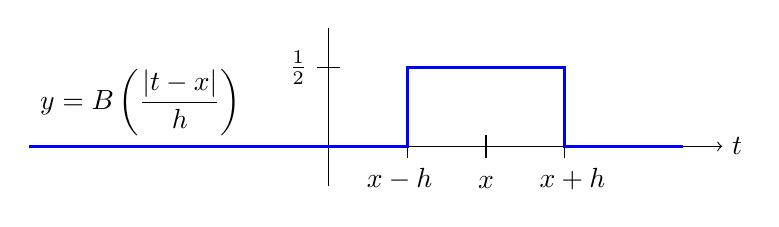
\begin{tikzpicture}
            \draw (0, -0.5) -- (0, 1.5);
            \draw (-0.15, 1) node[left] {$\frac12$} -- (0.15, 1);
            \draw[->] (-3.8, 0) -- (5, 0) node[right] {$t$};
            \draw (1, 0.15) -- (1, -0.15) node[below] {$x-h\;\;$};
            \draw (2, 0.15) -- (2, -0.15);
            \node at (2, -0.46) {$x$};
            \draw (3, 0.15) -- (3, -0.15) node[below] {$\;\;x+h$};
            \draw[very thick, blue] (-3.8, 0)  node[black, above right] {$y=B\left(\dfrac{|t-x|}h\right)$}-- (1, 0) -- (1, 1) -- (3, 1) -- (3, 0) --
            (4.5, 0);
\end{tikzpicture}


\bigskip
\textbf{Note:} $\text{Boxcar Kernel Smoother} = \text{Sliding Window Smoother}$

\textbf{Generalization:} Replace $B$ with another ``kernel'' function.

\end{frame}

\subsection{Kernel Functions}
\begin{frame}
    \frametitle{Kernel Functions}
    \setlength\parskip{0.75em}

    $K(x)$ is a \textbf{kernel function} if
    \begin{enumerate}
        \setlength\parskip{0.75em}
        \item $K(x)\geq 0$
        \item $K(-x)=K(x)$
        \item $\displaystyle \int_{-\infty}^\infty K(x)\,dx = 1$
    \end{enumerate}
\end{frame}

\begin{frame}
    \frametitle{Popular Kernels}
    \begin{enumerate}
        \setlength\parskip{0.75em}
        \item Boxcar: $$B(x) = \dfrac12\One_{(-1, 1)}(x)$$
        \item Triangular: $$T(x) = (1 - |x|)\One_{(-1, 1)}(x)$$
        \item Epanechnikov: $$E(x) = \dfrac34(1-x^2)\One_{(-1, 1)}(x)$$
        \item Gaussian: $$G(x) = \dfrac1{\sqrt{2\pi}}e^{-x^2/2}$$
    \end{enumerate}
\end{frame}

\begin{frame}
    \frametitle{Popular Kernels}
    \begin{center}
    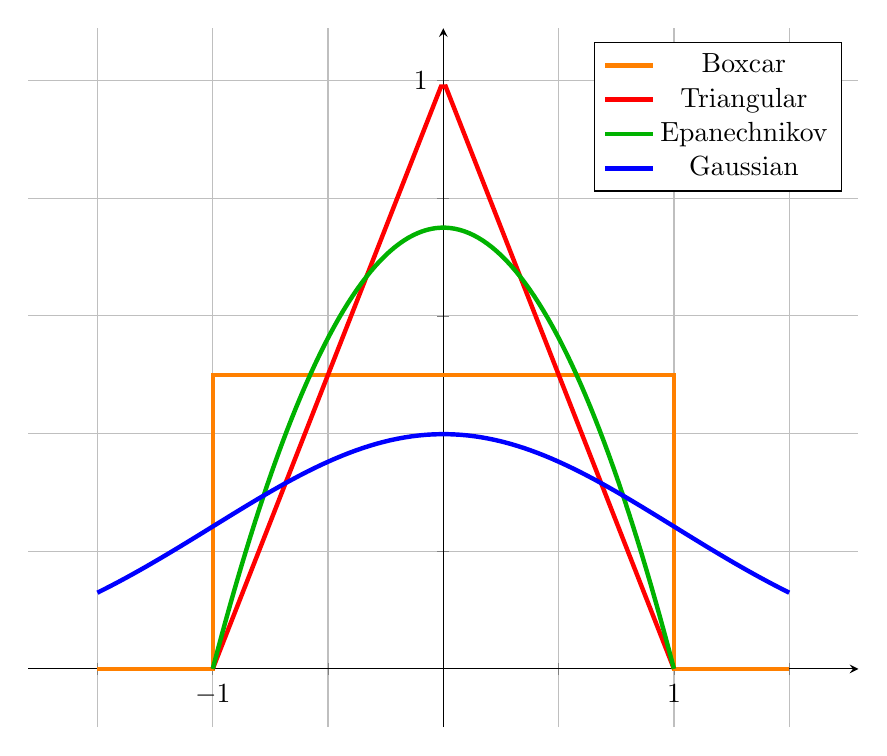
\begin{tikzpicture}
        \begin{axis}[grid=both,
                    axis lines=middle,
                    width=\textwidth,
                    xtick={-1.5, -1, -0.5, 0, 0.5, 1, 1.5},
                    xticklabels={{}, $-1$, {}, {}, {}, $1$},
                    ytick={0.2, 0.4, 0.6, 0.8, 1},
                    yticklabels={{}, {}, {}, {}, $1$},
                    enlargelimits]

        \addplot[orange, ultra thick] coordinates {
            (-1.5,0)
            (-1,0)
            (-1,0.5)
            (1,0.5)
            (1,0)
            (1.5, 0)
        };
        \addlegendentry{Boxcar};

        \addplot[red, ultra thick, domain=-1:1, samples=100]  {1 - abs(x)};
        \addlegendentry{Triangular};

        \addplot[black!30!green, ultra thick, domain=-1:1, samples=100]  {3*(1-x^2)/4};
        \addlegendentry{Epanechnikov};

        \addplot[blue, ultra thick, domain=-1.5:1.5, samples=100]  {exp(-x^2/2)/sqrt(2*pi)};
        \addlegendentry{Gaussian};
        \end{axis}
    \end{tikzpicture}
\end{center}
\end{frame}

\subsection{Kernel Smoothers}
\begin{frame}
    \frametitle{Kernel Smoothers}
\begin{definition}
    The \textbf{kernel smoother} associated to the data set
    \[
    \cD = \{(\vx_1,y_1),\;(\vx_1,y_1),\;\ldots,\;(\vx_n, y_n)\},
    \]
    a kernel function $K$, and a bandwidth $h>0$ 
    is the function $\hat{r}$ defined by
    \[
        \hat r(\vx) = \frac{\displaystyle\quad\sum_{i=1}^n y_i\,K\left(\frac{\|\vx - \vx_i\|}h\right)\quad}    
        {\displaystyle\sum_{i=1}^n K\left(\frac{\|\vx - \vx_i\|}h\right)}
    \]
\end{definition}

This is a \textbf{weighted average} of $y_1,\ldots,y_n$ with $y_i$ having weight $$w_i=K\left(\dfrac{\|\vx - \vx_i\|}h\right).$$
\end{frame}
\subsection{Examples}
\begin{frame}
    \frametitle{Comparison of Regression Models}
    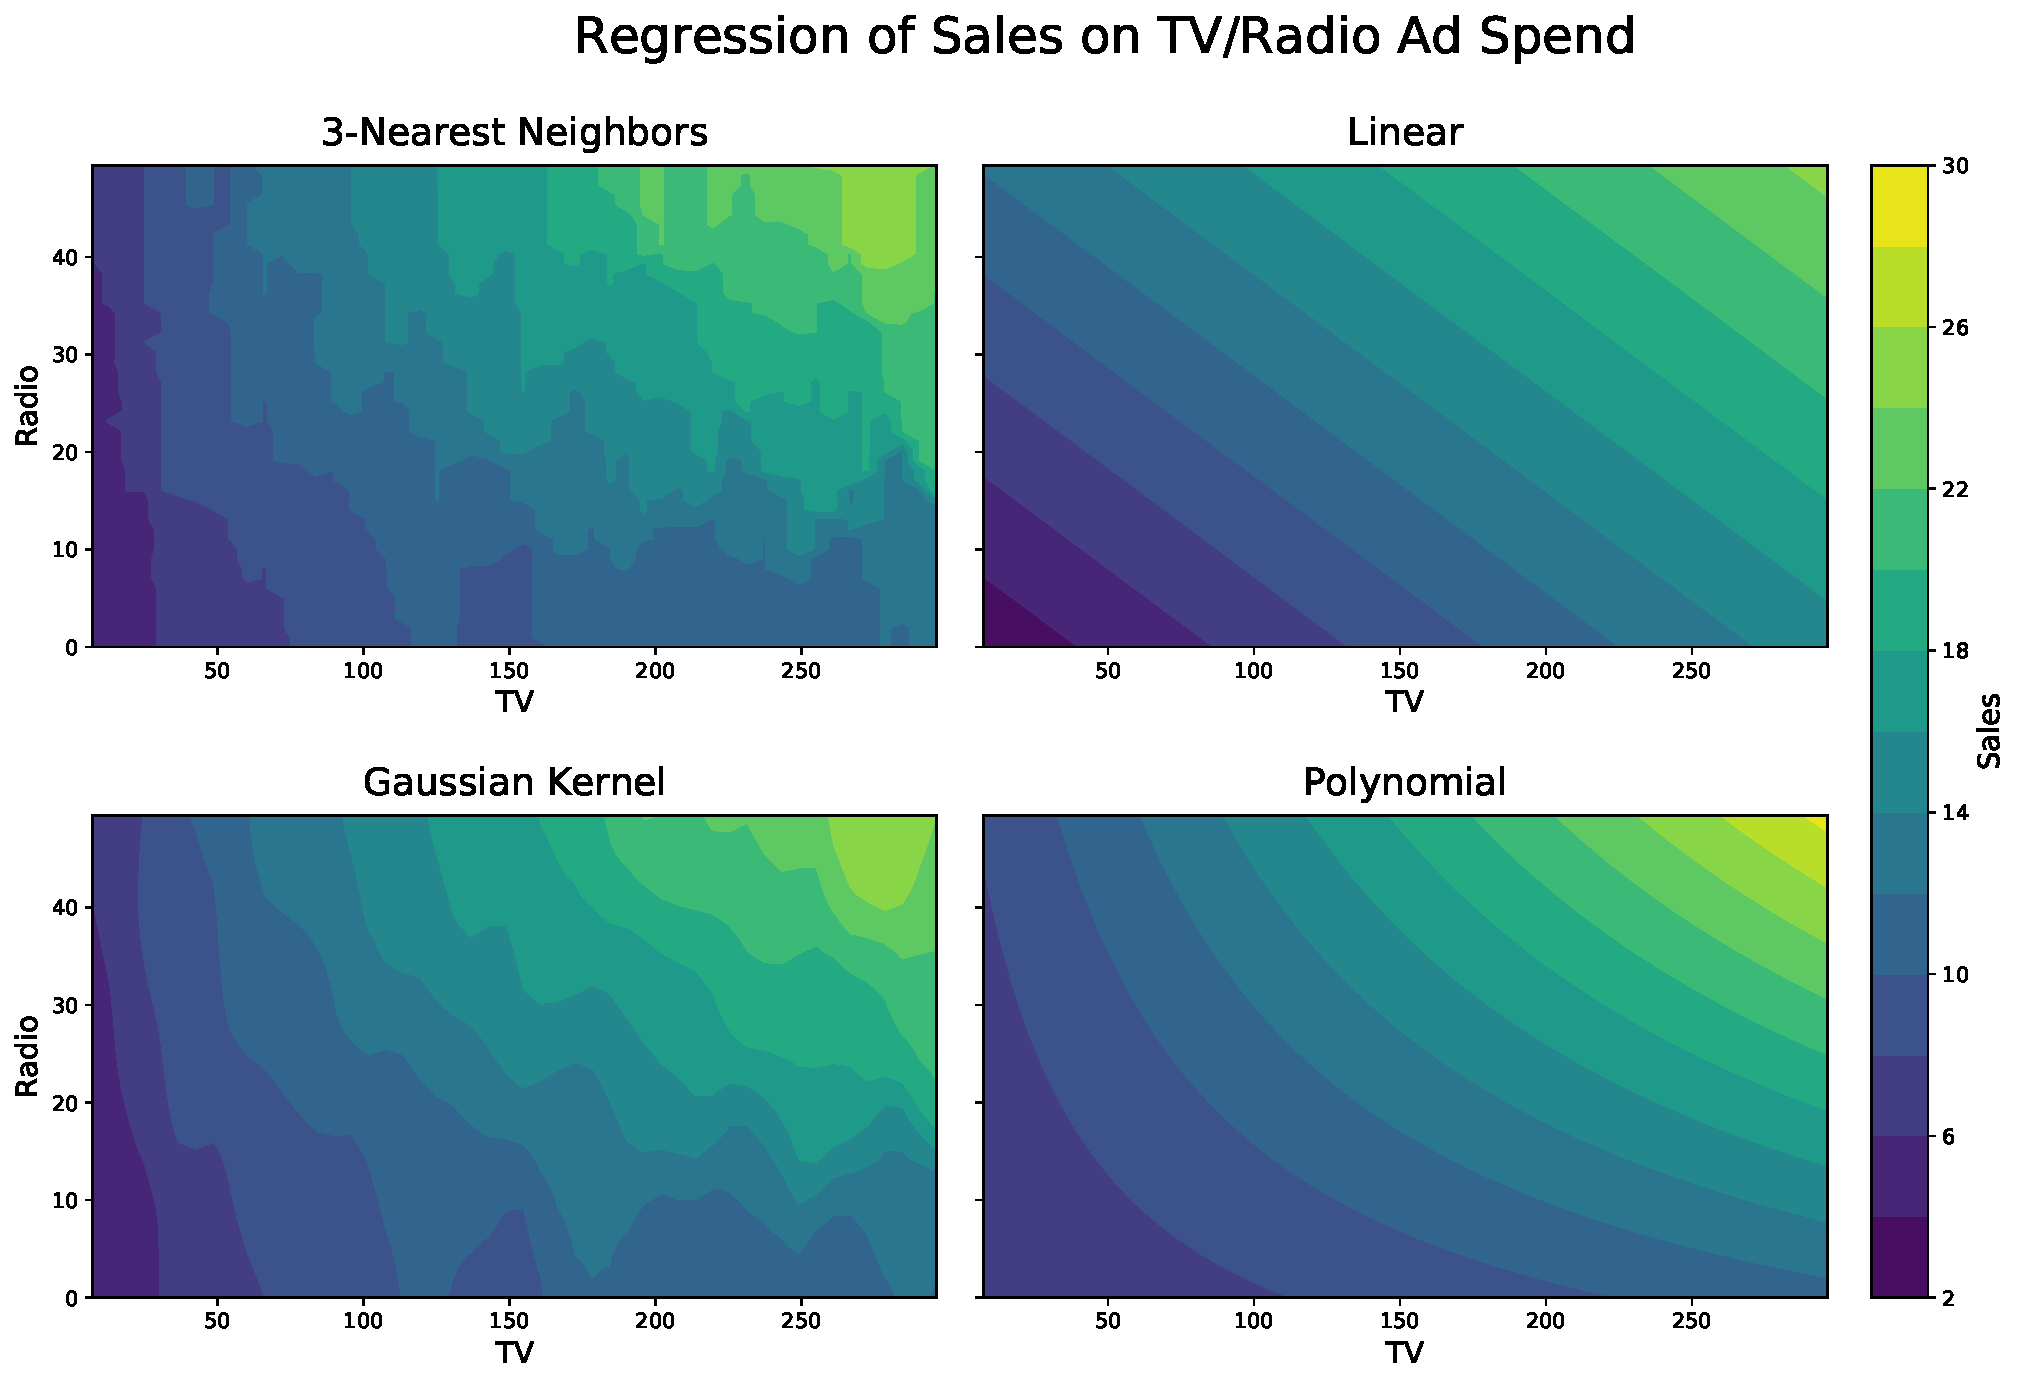
\includegraphics[scale=0.32]{advertising.pdf}
\end{frame}

\begin{frame}
    \setlength\parskip{0.75em}

    \begin{center}
    \begin{tabular}{rcc}
        \textbf{Model} & \textbf{Training MSE} & \textbf{Testing MSE}\\[1ex]\hline
        Linear Regression & 2.10 & 5.78\\[1ex]
        Polynomial Regression & 0.51 & 2.51\\[1ex]
        k-Nearest Neighbors ($k=3$) & 0.49 & 1.82\\[1ex]
        Gaussian Kernel ($h=6$) & 0.21 & 1.13\\\hline
    \end{tabular}
\end{center}

\begin{itemize}
    \setlength\parskip{0.75em}

    \item \texttt{advertising.csv}
    \item TV, Radio, and Sales columns only
    \item 160 training samples, 40 testing samples
\end{itemize}


    

\end{frame}
\end{document}